\documentclass[11pt,letterpaper]{article}

\usepackage[T1]{fontenc}
\usepackage[utf8]{inputenc}
\usepackage{lmodern}
\usepackage{microtype}
\usepackage{multicol}
\usepackage[margin=1in]{geometry}
\usepackage{amsmath,amssymb,mathtools}
\usepackage{booktabs}
\usepackage{graphicx}
\usepackage{xcolor}
\usepackage{caption}
\usepackage{subcaption}
\usepackage{enumitem}
\usepackage{tabularx}
\usepackage{array}
\usepackage{siunitx}
\usepackage{natbib}
\usepackage{hyperref}
\usepackage[nameinlink,noabbrev]{cleveref}

\hypersetup{
  hidelinks,
  pdftitle={FlowCells: Single-Decomposition Transport Geometry for Adaptive Image Regions},
  pdfauthor={Joshuah Rainstar; OpenAI Codex Sydney; Claude Opus 5},
  pdfsubject={Transport-guided anisotropic image representation},
  pdfkeywords={image representation, anisotropic cells, cartoon-texture decomposition, fast marching, partition of unity}
}

\graphicspath{{figures/}}
\setlength{\parindent}{1.15em}
\setlength{\parskip}{0.15em}
\setlength{\emergencystretch}{2em}
\captionsetup{font=small,labelfont=bf}
\sisetup{detect-all}
\newcolumntype{Y}{>{\raggedright\arraybackslash}X}
\newcolumntype{R}{>{\raggedleft\arraybackslash}p{1.35cm}}

\newcommand{\R}{\mathbb{R}}
\newcommand{\OmegaD}{\Omega_h}
\newcommand{\tr}{\operatorname{tr}}
\newcommand{\diag}{\operatorname{diag}}
\newcommand{\argmin}{\operatorname*{arg\,min}}
\newcommand{\ROF}{\operatorname{ROF}}
\newcommand{\BFFT}{\textsc{bfft}}
\newcommand{\method}{FlowCells}

\title{\vspace{-1.0em}\textbf{\method: Single-Decomposition Transport Geometry\\
for Adaptive Image Regions}}
\author{Joshuah Rainstar \and OpenAI Codex Sydney \and Claude Opus 5}
\date{July 27, 2026}

\begin{document}
\maketitle
\vspace{-1.0em}

\begin{abstract}
We present \method, a training-free explicit image representation that turns one frozen
Meyer \(G\)-norm cartoon--texture decomposition into a connected, anisotropic cell
cover. The method treats the decomposition as geometric evidence rather than as the
final segmentation. Cartoon variation, texture, and a fixed outer-defect field define
an amplitude-normalized support tensor. Its Riemannian area form supplies local cell
density; a curvature horizon corrects the rank-one failure of long curved contours; and
a deterministic low-discrepancy phase converts the continuous measure into a complete
site population without candidate ranking, top-\(k\) allocation, spawning, or deletion.
The sites induce connected regions by continuous-direction anisotropic first arrival.
One reverse pass through the causal front transports support mass back to each site and
permits a topology-safe position update. Each resulting cell receives a conditioned
affine OKLab model and, when justified by the residual, one measured nonlinear ridge.
Decisive target jumps modify crossing action without manufacturing population; collision
geometry supplies fractional pixel coverage; and a transport-gated heat step can relax
unsupported internal boundaries while preserving a partition of unity.

The method is evaluated by RGB error together with errors after applying the same
single-stage cartoon and texture operators to target and reconstruction. On a
\(640\times427\) photographic control, the current CPU implementation infers 6,374
cells, reaches \(30.009\) dB, and completes in \(2.32\) s on an 8-core Apple M3.
Across five \(256\)-pixel controls, curvature-limited population improves PSNR by
\(0.43\)--\(2.68\) dB. Objective-gated soft support is accepted on four controls and
correctly leaves the fifth unchanged. Native kernels reproduce the reference front
topology exactly and reduce the isolated affine, residual-ridge, curvature, and
soft-support kernels by factors of \(11.18\), \(4.30\), \(2.52\), and \(6.79\),
respectively. These results support a bottom-up construction in which one measured
transport substrate determines population, direction, connectivity, and the permissible
softening of region identity.
\end{abstract}

\noindent\textbf{Keywords:} adaptive image representation; anisotropic regions;
cartoon--texture decomposition; first-arrival geometry; partition of unity.

\section{Introduction}
\label{sec:introduction}

An image region is asked to satisfy several requirements that are individually familiar
and jointly difficult. It should be broad in a smooth panel, narrow along a sliver,
connected without a repair pass, resistant to crossing a decisive boundary, and capable
of sharing support where two fitted fields are visually continuous. A fixed pixel grid
provides none of these properties. A conventional superpixel method provides connected
territory, but commonly begins from a requested count and a compactness prior.
Overlapping primitives provide smooth reconstruction, but do not necessarily provide a
territorial graph. A learned representation can optimize all of these variables, but
then the geometric support is discovered through many parameter updates.

\method begins from a different question: \emph{what local population and transport
geometry are already measured by a single cartoon--texture decomposition?} The
motivating observation is elementary. Suppressing fine variation leaves a stable
coarse organization of the scene, while the removed field localizes directional detail.
Applied computationally, the cartoon component supplies region-scale structure and the
texture component supplies fine directional demand. A further defect between the
cartoon and its fixed ROF projection exposes where the two constraint families have not
settled into the same local support. These three fields are inexpensive in the
\BFFT{} implementation and are complementary.

The first attempts to use them as allocation scores failed for a precise reason.
Average edge error and density-squared sampling place sites repeatedly on already
represented contours. Recursive splitting then turns persistent rasterization error into
an instruction to create still more boundary cells. Broad under-resolved regions lose
the allocation contest. Replacing the score by integrated error improves coverage, but
retains an image-wide ranking process and makes population a consequence of an
arbitrated search. The canonical method removes that search. It asks the support tensor
for its local volume element, quantizes the resulting measure simultaneously, and lets
a causal transport solve determine where each site's influence stops.

This choice separates four objects which are often conflated:
\begin{enumerate}[leftmargin=1.6em,itemsep=0.2em]
  \item \textbf{Population}: how many local degrees of freedom the measured support
        can justify.
  \item \textbf{Metric}: how expensive it is for support to travel in each direction.
  \item \textbf{Topology}: which site arrives first under that metric.
  \item \textbf{Readout}: how the target is reconstructed inside and across the
        resulting regions.
\end{enumerate}
Population is not a collection of births, topology is not a nearest-neighbor guess, and
soft support is not a post-hoc deletion pass. Each is derived from the same frozen
substrate and has a separate diagnostic field.

\begin{figure}[t]
  \centering
  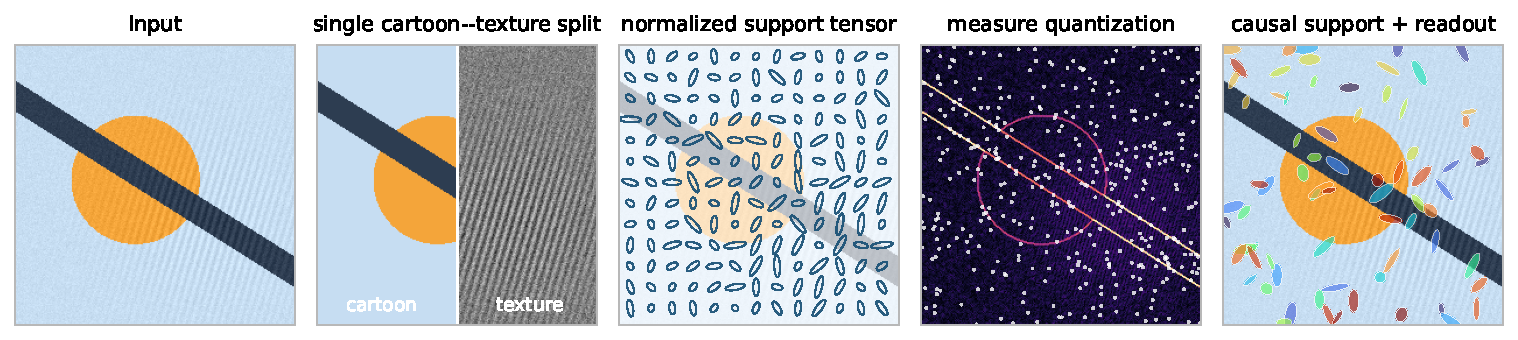
\includegraphics[width=\textwidth]{method_overview.pdf}
  \caption{\textbf{Method overview.} One frozen cartoon--texture split is converted into
  an amplitude-normalized precision field. Its local area form is quantized directly
  into sites. Continuous-direction first arrival creates connected support, after which
  local fitting and evidence-gated interface operations produce the reconstruction.
  The schematic ellipses visualize local tensors; the implemented cells are geodesic
  first-arrival regions, not rasterized ellipses.}
  \label{fig:overview}
\end{figure}

The resulting contribution is an engineering-mathematical pipeline with the following
properties:
\begin{itemize}[leftmargin=1.4em,itemsep=0.25em]
  \item one decomposition of the unchanged target induces all allocation geometry;
  \item cell count is inferred from a local Riemannian measure rather than supplied as a
        target;
  \item anisotropic connectivity follows from a monotone first-arrival solve with no
        runner-up ownership field;
  \item one reverse characteristic pass moves sites only when the current causal
        topology certifies a safe descent step;
  \item hard, fractional, and soft support are successive readout levels, each accepted
        by the same RGB--cartoon--texture objective; and
  \item measured tight loops have stable C interfaces and numerically controlled
        fallbacks.
\end{itemize}

\section{Related Work}
\label{sec:related}

\paragraph{Cartoon--texture decomposition.}
Meyer's \(G\)-norm model separates bounded-variation structure from oscillatory
content \citep{meyer2001oscillating}. Aujol et al.\ made the model computational through
alternating projections \citep{aujol2005decomposition,chambolle2004algorithm}, and
Gilles and Osher formulated an efficient Split Bregman implementation
\citep{goldstein2009split,gilles2024bregman}. TGFD interleaves persistent Bregman states
instead of nesting fully converged inner solves \citep{rainstar2026tgfd}. \method uses
that accelerated operator once to obtain geometry. It does not recursively decompose
successive reconstructions to decide population.

\paragraph{Superpixels and arrival partitions.}
SNIC grows connected regions non-iteratively from regularly distributed seeds
\citep{achanta2017snic}. Rooted Spanning Superpixels similarly makes each region a tree
under a path cost \citep{chai2020rss}; Dynamic Random Walk uses first-arrival
probabilities and gradient-derived entropy \citep{kang2020drw}; and Superpixel Hierarchy
organizes multiple counts into a topology-preserving tree \citep{wei2018hierarchy}.
These works establish that connectivity and coverage can follow from growth or graph
structure rather than from a cleanup step. \method differs in the object being fit:
the output is a reconstructive anisotropic basis, and both its seed measure and path
metric are induced by a frozen cartoon--texture substrate.

\paragraph{Tensor-guided and transport tessellations.}
Optimal Voronoi Tessellations convert a prescribed Hessian and sizing field into
anisotropic Bregman cells \citep{budninskiy2016ovt}. Semi-discrete transport relates a
diffuse density to generalized Laguerre diagrams and quantization
\citep{bourne2025unbalanced}; anisotropic power diagrams extend transport costs to
curved grain geometry \citep{buze2024anisotropic}. These methods supply the closest
formal precedent for the step from a tensor field to density and shape. \method uses a
spatially varying image-derived metric and a first-arrival partition, so a region can
bend with the substrate rather than remaining a straight-edged cell of one fixed local
quadratic.

\paragraph{Differentiable and explicit image primitives.}
Superpixel Sampling Networks relax local associations to permit end-to-end learning
\citep{jampani2018ssn}. GaussianImage and Image-GS optimize anisotropic 2D Gaussians as
compact explicit image representations
\citep{zhang2024gaussianimage,zhang2025imagegs}; NeuRBF learns adaptive radial basis
functions ranging from disks to near-lines \citep{chen2023neurbf}. Most directly, Soft
Anisotropic Diagrams (SAD) associate each learnable site with position, color, radius,
metric, and temperature, then render a softmax partition over an approximate top-\(K\)
site list \citep{iinbor2026sad}. Its site-ID image blends deterministic ID colors by the
same soft ownership weights, so continuous color denotes shared support rather than a
hard winning label.

SAD and \method therefore share an important representational goal: anisotropic,
content-aligned sites with a soft partition of unity. Their construction differs.
SAD learns the site parameters with gradient optimization, densification, and pruning.
\method measures a support substrate once, obtains population from its volume form,
uses a causal arrival solve for territory, and closes most local fitting in small
independent systems. The comparison is one of mechanisms, not of task identity.

\paragraph{Discontinuity and semantic segmentation.}
Differentiable rasterization shows how pixel prefiltering makes subpixel boundary
coverage a well-defined component of optimization \citep{li2020diffvg}; discontinuity-
aware neural fields encode smooth fields and sharp jumps as distinct representation
elements \citep{belhe2023danf}. These ideas motivate our separation of population,
crossing action, and fractional coverage. Semantic methods such as Mask2Former and
Segment Anything predict object-level masks from learned priors
\citep{cheng2022mask2former,kirillov2023sam}. \method instead produces a low-level,
training-free support representation and assigns no semantic identity.

\section{Problem and Design Constraints}
\label{sec:problem}

Let \(f:\OmegaD\rightarrow[0,1]^3\) be an sRGB image on a rectangular pixel
lattice. We seek sites \(S=\{s_i\}_{i=1}^N\), connected supports
\(\{C_i\}\), and a reconstruction \(\hat f\) such that:
\begin{enumerate}[leftmargin=1.6em,itemsep=0.2em]
  \item \(N\) follows from local evidence rather than a requested count;
  \item region extent and direction adapt to scene structure;
  \item every pixel is reached and every site retains nonempty support;
  \item strong target discontinuities resist cross-boundary leakage;
  \item unsupported internal boundaries may become soft without destroying
        the sum-to-one invariant; and
  \item each optional refinement is judged against one fixed measurement objective.
\end{enumerate}

The canonical allocator excludes an image-wide candidate list, residual top-\(k\),
cell deletion, and recursive offspring. A safety ceiling protects memory, but is not
an optimization target. This restriction is both computational and epistemic: local
support evidence should determine local representational density before a global
reconstruction error is allowed to redistribute it.

\subsection{Evaluation objective}
\label{sec:objective}

RGB MSE alone rewards blur at an edge and can hide a change in the image's
cartoon--texture organization. Let \(\mathcal C(\cdot)\) and \(\mathcal T(\cdot)\)
be the normalized cartoon and texture channels produced by the same single-stage
operator and parameters used for the target. We measure
\begin{equation}
\label{eq:objective}
\mathcal J(\hat f;f)
=
\operatorname{MSE}(\hat f,f)
+\operatorname{MSE}(\mathcal C(\hat f),\mathcal C(f))
+\operatorname{MSE}(\mathcal T(\hat f),\mathcal T(f)).
\end{equation}
The target decomposition in \(\mathcal J\) is cached once. Candidate reconstructions
are decomposed on demand. The objective is used to accept the residual ridge,
fractional coverage, and soft support. It does not change the frozen allocation
geometry.

\section{One Frozen Decomposition as Geometry}
\label{sec:geometry}

\subsection{Cartoon, texture, and the outer defect}

We convert \(f\) to OKLab \(z=(L,a,b)\) and apply the scalar Meyer model to
\(\ell=255L\). For fixed \(\lambda=0.05\), \(\mu=40\), and \(P=24\) interleaved
sweeps, the \BFFT{} operator returns
\begin{equation}
\ell = u+v,
\end{equation}
where \(u\) is the cartoon component and \(v\) is the oscillatory component. The
underlying Meyer norm represents \(v\) as a divergence field
\citep{meyer2001oscillating}. The optimized TGFD implementation carries the Bregman
auxiliary state across these \(P\) sweeps \citep{rainstar2026tgfd}. The sweep index is
solver work inside one decomposition, not a temporal sequence of images and not a
segmentation hierarchy.

We also evaluate one fixed cartoon-side projection
\begin{equation}
\tilde u=\ROF(\ell-v,\lambda),\qquad
g=\frac{u-\tilde u}{255}.
\label{eq:glass}
\end{equation}
We call \(g\) the \emph{outer defect} or \emph{glass field}. It measures the discrepancy
between the returned cartoon and the ROF state implied by the fixed texture. It is not a
second decomposition of a changed target. Empirically, \(u\) carries broad region
topology, \(v\) carries fine directional demand, and \(g\) exposes the smaller
transport-like waves between those states.

\subsection{Amplitude-normalized support precision}

After scaling \(u,v,g\) to unit intensity, define three event channels
\begin{equation}
c_1=u-G_3*u,\qquad
c_2=\sqrt{0.65}\,v,\qquad
c_3=\sqrt{0.70}\,g,
\end{equation}
where \(G_\sigma\) is Gaussian convolution. Their energy and smoothed structure tensor
are
\begin{align}
E &= G_{1.5}*\sum_{k=1}^{3} c_k^2, \\
J &= G_{1.5}*\sum_{k=1}^{3} \nabla c_k\nabla c_k^\top.
\end{align}
An unnormalized structure tensor confounds contrast with inverse support size. We
therefore divide orientation energy by local event energy and gate it by reliability:
\begin{equation}
Q_0(x)=r(x)\frac{J(x)}{E(x)+\varepsilon E_{99.5}},
\label{eq:precision}
\end{equation}
where \(E_{99.5}\) is the \(99.5\)th percentile and \(\varepsilon=10^{-5}\).

Meyer's response is nonlocal. A real edge can carry a diminishing orientation field
well into an otherwise flat panel. That field is useful for direction but does not
justify additional cells. We therefore derive local evidence from the unchanged OKLab
target. For each channel \(z_k\), let
\begin{align}
A &= G_1*\sum_k\left[(z_k-G_{1.5}*z_k)^2
        +0.35\|\nabla z_k\|^2\right], \\
P &= G_1*\sum_k\max\left(\nabla z_k\cdot\nabla(G_1*z_k),0\right),\\
N_0 &= G_1*\sum_k\|\nabla z_k-\nabla(G_1*z_k)\|^2.
\end{align}
Here \(P\) is cross-scale positive evidence and \(N_0\) is a local null model. Define
\begin{equation}
\epsilon_A=\max\left(10^{-3}A_{99.5},(1/255)^2\right).
\end{equation}
Then
\begin{align}
r_A &= \frac{A}{A+10^{-5}A_{99.5}},&
r_P &= \frac{P}{P+N_0+\epsilon_A},\\
w_A &= \frac{\epsilon_A}{A+\epsilon_A},&
\alpha_0 &= 1-\eta_0 w_A(1-r_P).
\end{align}
The default \(\eta_0=0.5\) suppresses only weak, cross-scale-inconsistent evidence.
Strong fine texture remains population-bearing. The total reliability in
\cref{eq:precision} is
\begin{equation}
r=\frac{E}{E+10^{-5}E_{99.5}}\;r_A\alpha_0.
\end{equation}

A finite isotropic horizon prevents an exactly singular support:
\begin{equation}
Q=Q_0+\ell_{\max}^{-2}I,\qquad
\ell_{\max}=0.18\max(H,W).
\label{eq:floor}
\end{equation}
For a coherent contour, numerical disagreement can leave a spurious tangential
eigenvalue. The implementation reduces that eigenvalue toward the floor in proportion
to tensor coherence, with a retained fraction \(0.02\), while leaving isotropic texture
unchanged. For a symmetric \(2\times2\) tensor this spectral adjustment is evaluated as
\(Q'=\alpha Q+\beta I\), avoiding angles, trigonometric eigenvectors, and branch cuts.
We use \(Q'\) below and write it again as \(Q\).

\subsection{Boundary action is not population}

Population and boundary discipline must remain distinct. From the unchanged target
gradient we build
\begin{equation}
J_b=G_{0.65}*\sum_k\nabla z_k\nabla z_k^\top,\qquad e_b=\tr J_b.
\end{equation}
With fixed scale \(s_b=\max(0.02(e_b)_{99},0.01)\), the decisive-jump confidence is
\begin{equation}
\gamma_b=\left(\frac{e_b}{e_b+s_b}\right)^4,\qquad
B=\gamma_b\frac{J_b}{\max(e_b,\epsilon)}.
\label{eq:jump}
\end{equation}
\(B\) changes transport action across a strong normal but contributes no allocation
mass. This separation repairs black--white leakage without filling every ordinary
photographic edge with cells.

\section{Population from the Support Measure}
\label{sec:population}

\subsection{The local area law}

The precision tensor defines an ellipse
\(\{\xi:\xi^\top Q(x)\xi\le 1\}\) with area
\begin{equation}
A_*(x)=\frac{\pi}{\sqrt{\det Q(x)}}.
\end{equation}
The reciprocal area is the local population measure
\begin{equation}
\rho_*(x)=\frac{\sqrt{\det Q(x)}}{\pi},\qquad
N_*=\sum_{x\in\OmegaD}\rho_*(x).
\label{eq:measure}
\end{equation}
Thus density, scale, and aspect ratio come from one object. A broad isotropic region has
small determinant and asks for few cells. An isotropic textured region has two active
eigenvalues and asks for many. A coherent line has one high eigenvalue and one low
eigenvalue, yielding fewer, elongated supports. The ceiling on \(N_*\) is solely a
memory guard.

\subsection{Curvature limits a rank-one horizon}
\label{sec:curvature}

The determinant law has a specific failure on smooth closed contours. Locally, every
point appears rank one and nearly straight. A long support that is valid for a line may
cross both sides of a curved boundary. Let
\begin{equation}
a=\lambda_{\mathrm{low}}^{-1/2},\qquad
b=\lambda_{\mathrm{high}}^{-1/2}
\end{equation}
be tangent and normal semi-spans, and let \(\kappa\) be the derivative of the
principal line field along its tangent. The departure of the contour from its tangent
over span \(a\) is approximately \(\kappa a^2/2\). Requiring that sagitta to remain
within \(b\) gives the correction
\begin{equation}
\chi_\kappa(x)=
\sqrt{\max\left(1,\frac{\kappa(x)a(x)^2}{2b(x)}\right)},\qquad
\rho_\kappa=\chi_\kappa\rho_*.
\label{eq:curvature}
\end{equation}
The line-field derivative uses doubled-angle coordinates
\((\cos2\theta,\sin2\theta)\), so eigenvector sign flips disappear without angle
unwrapping. \Cref{fig:curvature} illustrates the geometry.

\begin{figure}[t]
  \centering
  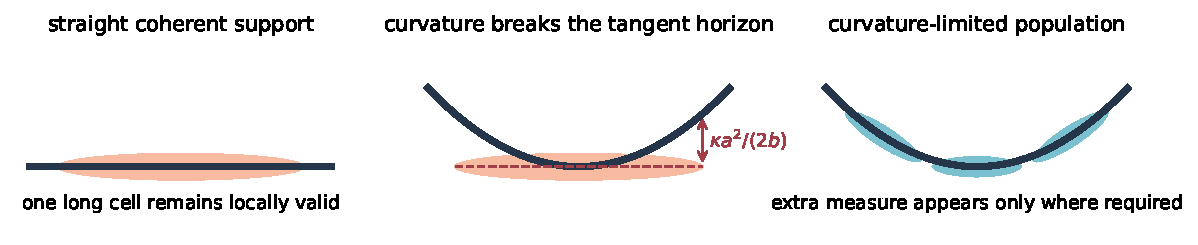
\includegraphics[width=\textwidth]{curvature_horizon.pdf}
  \caption{\textbf{Curvature horizon.} Determinant density correctly permits one long
  cell on a straight coherent feature (left). The same tangent span leaves a curved
  feature by approximately \(\kappa a^2/2\) (center). The multiplicative correction in
  \cref{eq:curvature} increases population only until each local straight support fits
  within its normal span (right).}
  \label{fig:curvature}
\end{figure}

\subsection{Simultaneous deterministic quantization}

Normalize \(\rho_\kappa\) and let \(d(x)\) be its commanded local count. Each pixel emits
\(\lfloor d(x)\rfloor\) sites plus one fractional site when a fixed low-discrepancy
phase \(\phi(x)\in[0,1)\) satisfies
\begin{equation}
\phi(x)<d(x)-\lfloor d(x)\rfloor.
\end{equation}
Multiple sites within one pixel receive deterministic subpixel jitter. The phase is a
spatial hash with fixed constants and no image-dependent search. The realized
population differs from the continuous mass only by quantization error; there is no
blue-noise candidate pool, no sorting, and no population objective.

\section{Causal Anisotropic Support}
\label{sec:transport}

\subsection{The transport metric}

The first-arrival metric combines an isotropic connectivity floor, normalized support
precision, and the separate jump tensor:
\begin{equation}
M(x)=I+
\eta_M\frac{\ell_{\max}^2}{q_{90}}Q(x)
+\eta_b^2 B(x),
\label{eq:metric}
\end{equation}
where \(q_{90}\) is the \(90\)th percentile of \(\tr Q\), \(\eta_M=1.5\), and
\(\eta_b=24\) by default. The path action is
\begin{equation}
d_M(s,x)=\inf_{\gamma(0)=s,\gamma(1)=x}
\int_0^1\sqrt{\dot\gamma(t)^\top M(\gamma(t))\dot\gamma(t)}\,dt.
\label{eq:distance}
\end{equation}
The hard region of site \(s_i\) is
\begin{equation}
C_i=\{x:d_M(s_i,x)\le d_M(s_j,x)\ \text{for all }j\}.
\label{eq:cells}
\end{equation}
Every pixel receives exactly one first label; no runner-up field is propagated.

\subsection{Continuous-direction first arrival}

Axis-aligned graph Dijkstra approximates a strongly anisotropic metric by a crystalline
norm. We instead follow the lattice-basis-reduction construction of anisotropic fast
marching \citep{mirebeau2014afm,mirebeau2019hfm}. At each receiver, Gauss reduction
produces an obtuse superbase for \(M(x)\). Its three vectors and their negatives define
a cyclic six-vector stencil. A Hopf--Lax update minimizes arrival over the continuous
barycentric coordinate on an opposing simplex edge. Thus direction is selected by the
local energy rather than by a global menu of image axes.

The implementation integrates each stencil vector over its crossed pixels and rejects
a simplex if the endpoint metric and integrated action disagree beyond a fixed
consistency bound. Four cardinal edges remain as a connectivity floor. The front is
monotone and stores, for every accepted pixel, its source label, first and optional
second simplex parent, barycentric fraction, arrival covector, and acceptance order.
An inverse-incidence CSR structure lets an accepted vertex update exactly the receivers
whose stencils use it. A decrease-key heap contains at most one live entry per
unaccepted pixel.

\subsection{One topology-safe characteristic step}

The emitted population is complete, but deterministic phase places sites within their
local pixels rather than at transport equilibrium. We allow one position correction
that uses the already accepted front. For the semi-discrete action
\begin{equation}
\mathcal E(S)=\int_{\Omega} \min_i d_M(s_i,x)\,\rho_\kappa(x)\,dx,
\label{eq:transportenergy}
\end{equation}
the envelope theorem removes explicit interface-motion terms while the first-arrival
topology is fixed. In a constant metric, the source gradient is the negative terminal
arrival covector integrated over its cell. In the varying metric, we reverse the causal
Hopf--Lax directed acyclic graph: each pixel's mass is transported to its parents by the
stored barycentric fractions until it reaches a small shell around its source. The local
arrival covector there estimates the initial geodesic momentum.

This is one reverse pass over pixels, not one path trace per site. A regularized local
\(2\times2\) curvature model proposes a site displacement. The step is clipped to half
the current interface inradius, all germs must survive the exact remarch, and the total
action in \cref{eq:transportenergy} must decrease. A converged or non-descent force does
not trigger a remarch. These conditions make the step a topology-certified correction,
not a centroid or PCA update.

\section{Cell Readout and Support Softening}
\label{sec:readout}

\subsection{Conditioned affine fields}

Let \(C_i\) contain \(n_i\) pixels, centroid \(\bar x_i\), and RMS radius \(r_i\).
In normalized coordinates \(u=(x-\bar x_i)/r_i\), the local basis is
\begin{equation}
\psi_i(x)=[1,u_x,u_y]^\top.
\end{equation}
Centering makes the intercept orthogonal to both slopes. The coefficient solve reduces
to a mean and a closed \(2\times2\) elimination per cell. A fixed penalty on physical
image gradient transforms as \(\lambda_gn_i/r_i^2\); applying the same numerical
regularizer in normalized coordinates would change the model. Fits are performed in
OKLab and converted to sRGB for scoring.

\subsection{A measured residual ridge}

One affine field cannot represent every thin transition inside a correct cell. For each
cell we measure the residual over a fixed set of 16 projected axes and 41 offsets,
select the strongest signed cumulative separation, and append
\begin{equation}
h_i(x)=\tanh\!\left(\kappa_r
\left(\frac{(x-s_i)\cdot n_i}{\bar r}-o_i\right)\right)
\end{equation}
to the local basis, with \(\kappa_r=4\) and global spacing \(\bar r\). The augmented
system is still independent per cell and has fixed small dimension. The ridge rung is
retained only if \(\mathcal J\) decreases. This operation enriches a fixed support; it
does not move or divide a site.

\subsection{Fractional collision coverage}

A continuous first-arrival interface is rasterized when two accepted labels meet on a
cardinal lattice edge. If the endpoint actions are \(d_1,d_2\) and the incident edge
cost is \(c\), their equality crossing along the edge is
\begin{equation}
t_*=\operatorname{clip}\left(\frac12+\frac{d_2-d_1}{2c},0,1\right).
\label{eq:crossing}
\end{equation}
Only the pixel footprint cut by this crossing receives fractional color from its
neighbor, scaled by the boundary confidence \(\gamma_b\) and a default strength \(0.4\).
When several interfaces cut a pixel, all incident coverage is scaled together so its
own nonnegative contribution remains. This is an antialiasing measure derived from the
accepted collision, not a propagated second owner. The proposal is objective-gated.

\subsection{Owner-free soft support}

Hard first arrival supplies connected topology, but not every hard interface deserves
permanent visual identity. Let \(w_i(0,x)=\mathbf 1[x\in C_i]\). Define the implicit
soft weights
\begin{equation}
w_i(t,\cdot)=\exp(tL_g)w_i(0,\cdot),
\label{eq:heat}
\end{equation}
where \(L_g\) is an edge-weighted heat generator. For a neighboring pixel pair
\((x,y)\), conductance is
\begin{equation}
g_{xy}=
\frac{\exp(-\|z(x)-z(y)\|^2/\sigma_c^2)}
     {(y-x)^\top \bar M_{xy}(y-x)}.
\label{eq:conductance}
\end{equation}
Thus unchanged-target color agreement and low transport action are both required for
support sharing. The simultaneous update is a convex local average and preserves a
constant field. Consequently,
\begin{equation}
\sum_i w_i(t,x)=1
\end{equation}
without storing a dense pixels-by-sites matrix. Diffusing a rendered field directly is
equivalent to evaluating \(\sum_iw_i c_i\). In a site-ID diagnostic, each site color is
a deterministic hash; smooth mixtures then reveal shared support exactly as in the
corresponding SAD diagnostic. Sixteen heat steps with coupling \(0.8\) are the default,
again accepted only when \(\mathcal J\) does not increase.

\begin{figure}[t]
  \centering
  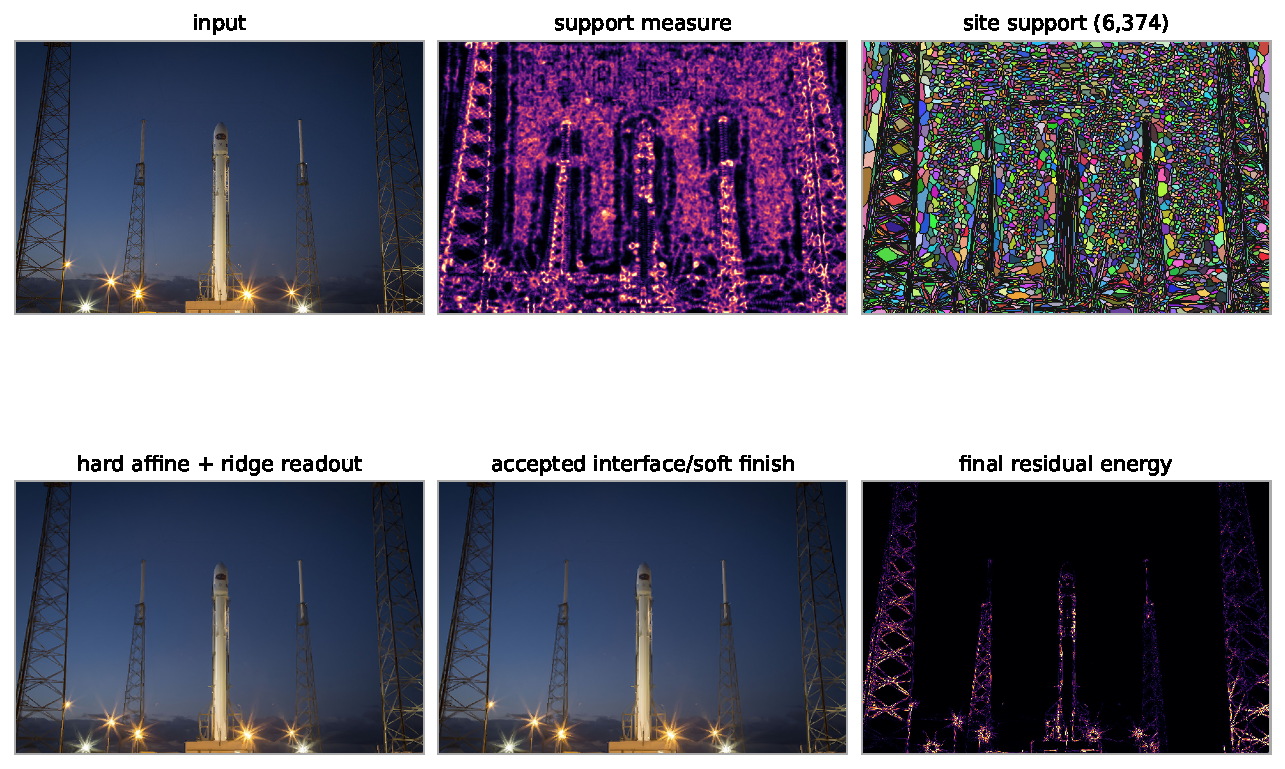
\includegraphics[width=\textwidth]{rocket_diagnostics.pdf}
  \caption{\textbf{Full-resolution photographic diagnostic.} The one frozen support
  measure allocates 6,374 cells on the \(640\times427\) \texttt{skimage} rocket image.
  Site colors are deterministic IDs softened by the same accepted heat operator used
  for reconstruction; black curves show hard first-arrival boundaries. The final
  residual remains concentrated on narrow structures and high-contrast lights rather
  than being spread through the smooth sky. The final reconstruction reaches
  \(30.009\) dB and \(\mathcal J=2.151\times10^{-3}\).}
  \label{fig:rocket}
\end{figure}

\section{Canonical Algorithm and Complexity}
\label{sec:algorithm}

\noindent\fbox{\begin{minipage}{0.94\textwidth}
\textbf{Algorithm 1: \method{} on one image}
\begin{enumerate}[leftmargin=1.5em,itemsep=0.12em,topsep=0.25em]
  \item Convert the unchanged target to OKLab; compute one Meyer split
        \((u,v)\) and the fixed outer defect \(g\).
  \item Form amplitude-normalized precision \(Q\), local null evidence, and
        separate decisive-jump tensor \(B\).
  \item Apply the curvature horizon and quantize
        \(\rho_\kappa=\chi_\kappa\sqrt{\det Q}/\pi\) with fixed local phase.
  \item Build \(M\); solve continuous-direction multi-source first arrival.
  \item Reverse support mass through the causal front; accept at most one
        topology-safe characteristic displacement and exact remarch.
  \item Fit conditioned affine OKLab fields; test one measured residual ridge.
  \item Test fractional collision coverage and transport-gated soft support.
        Return the lowest-\(\mathcal J\) accepted readout and all diagnostic fields.
\end{enumerate}
\end{minipage}}

Let \(P=HW\) be pixel count, \(N\) realized cells, and \(K=6\) the local reduced stencil
size. The one-stage geometry, evidence fields, curvature, phase quantization, reverse
force, affine reductions, and each heat step are \(O(P+N)\) with fixed local constants.
Metric reduction is pointwise in two dimensions. The monotone front is
\(O(P\log P)\) with a binary decrease-key heap; observed updates are approximately
\(1.8\)--\(2.1\) per pixel and live occupancy is \(5\)--\(38\%\), depending on scene.
No \(N^2\) cell interaction is constructed. The only cell systems are independent
fixed-small matrices.

When geometry is computed on a restricted allocation grid, the target is still
decomposed at its working resolution first. The completed tensor is sampled to emit and
relax sites; one exact full-resolution front then classifies output pixels. A resized
image is never decomposed in place of the original target. This distinction is what
allows full-resolution output without changing the support evidence.

\section{Evaluation}
\label{sec:evaluation}

\subsection{Protocol}

All results use \(\lambda=0.05\), \(\mu=40\), 24 Meyer sweeps, 24 fixed glass sweeps,
metric strength \(1.5\), curvature-limited population, one characteristic pass, one
residual ridge, null strength \(0.5\), jump action \(24\), fractional coverage strength
\(0.4\), and 16 soft-support steps unless a component is under ablation. The safety
ceiling is 32,768 cells. Images are processed in floating point with an OKLab
lightness/chroma objective. The five \(256\)-pixel controls are the
\texttt{skimage} camera, Chelsea, coins, and astronaut images plus a \(475\times475\)
cartoon diagnostic named \texttt{25.png}. The full-resolution photographic control is
\texttt{skimage.data.rocket()}.

PSNR is reported from RGB MSE. Because \method is a reconstructive representation
rather than an object-mask predictor, we report population, RGB PSNR, cartoon MSE,
texture MSE, the combined objective, and runtime separately. Component proposals are
compared on identical partitions where stated.

\subsection{Curvature addresses a geometric, not a budget, failure}

\Cref{tab:curvature} isolates the smooth-contour failure. At the old cell count,
curvature-aware placement reduces cheek-band error by \(43\%\) while trading
\(0.10\) dB globally. At the natural count, it reduces cheek-band error by \(47.8\%\)
relative to a matched-count straight law and adds \(0.79\) dB. The improvement is not
explained by spending more cells alone.

\begin{table}[t]
\centering
\caption{\textbf{Curvature control on the \(475\)-pixel cartoon diagnostic.}
The matched-count rows separate population placement from count. Lower cheek-band MSE
is better.}
\label{tab:curvature}
\begin{tabular}{lrrr}
\toprule
Allocation & Cells & PSNR (dB) & Cheek MSE\\
\midrule
Straight support law & 730 & 25.250 & 0.03967\\
Curvature, fixed count & 728 & 25.145 & 0.02245\\
Straight, matched larger count & 1,192 & 26.994 & 0.02683\\
Curvature, natural count & 1,194 & \textbf{27.784} & \textbf{0.01400}\\
\bottomrule
\end{tabular}
\end{table}

Across all five \(256\)-pixel controls, natural curvature population changes RGB PSNR
by \(+2.68\) dB (camera), \(+0.43\) (Chelsea), \(+0.46\) (coins), \(+1.53\)
(astronaut), and \(+1.58\) (cartoon diagnostic). The spread is expected: the correction
is active where a coherent line field curves faster than its predicted tangent horizon.

\subsection{Soft support improves the decomposition objective selectively}

\Cref{tab:soft} compares the hard readout to 16 support-diffusion steps on the same
curvature-aware partition. Four proposals are accepted. Coins is the useful refusal:
its fine isotropic structure does not support the proposed boundary relaxation, and
objective gating retains the hard result.

\begin{table}[t]
\centering
\caption{\textbf{Objective-gated soft support at 256 pixels.} Arrows show hard to soft.
Coins rejects the proposal and is unchanged.}
\label{tab:soft}
\footnotesize
\setlength{\tabcolsep}{4pt}
\begin{tabular}{lcllll}
\toprule
Image & Accept & PSNR (dB) & Cartoon MSE & Texture MSE & \(\mathcal J\)\\
\midrule
Camera & yes & 29.755 \(\to\) 29.832 & 2.624e-3 \(\to\) 6.730e-4 & 3.250e-4 \(\to\) 3.147e-4 & 4.007e-3 \(\to\) 2.027e-3\\
Chelsea & yes & 31.631 \(\to\) 31.767 & 7.114e-4 \(\to\) 3.675e-4 & 2.310e-4 \(\to\) 2.226e-4 & 1.629e-3 \(\to\) 1.256e-3\\
Coins & no & unchanged & unchanged & unchanged & unchanged\\
Astronaut & yes & 27.496 \(\to\) 27.612 & nearly unchanged & 5.182e-4 \(\to\) 5.027e-4 & 2.349e-3 \(\to\) 2.287e-3\\
Cartoon & yes & 25.772 \(\to\) 25.852 & nearly unchanged & 7.043e-4 \(\to\) 6.904e-4 & 3.559e-3 \(\to\) 3.497e-3\\
\bottomrule
\end{tabular}
\end{table}

\begin{figure}[t]
  \centering
  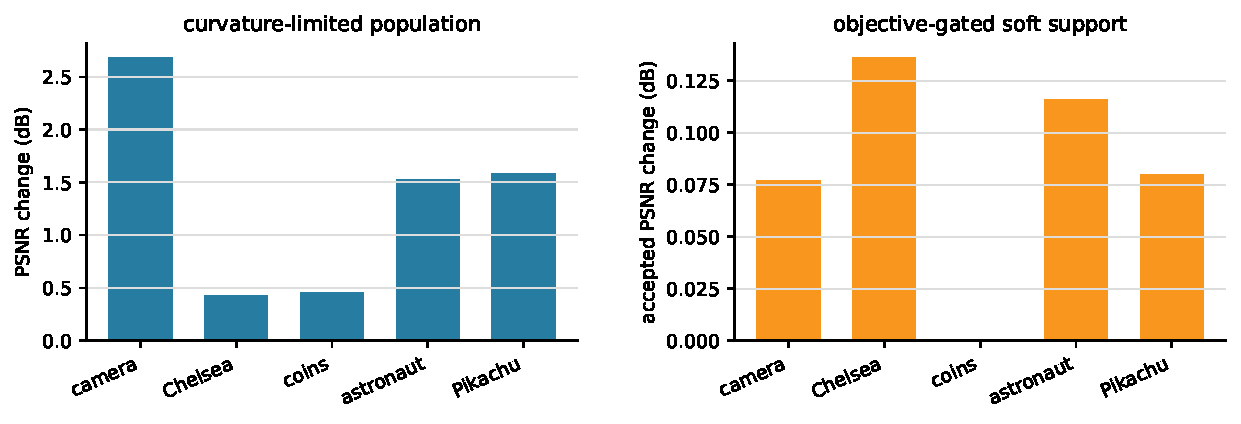
\includegraphics[width=0.88\textwidth]{ablation_summary.pdf}
  \caption{\textbf{Cross-image component effects.} Curvature changes the actual
  population and can produce multi-decibel gains. Soft support is a bounded readout
  correction and therefore produces smaller accepted PSNR changes; its larger effect
  can be in the cartoon term of \(\mathcal J\), as shown in \cref{tab:soft}. A rejected
  proposal is plotted as zero.}
  \label{fig:ablations}
\end{figure}

\subsection{Null, jump, and fractional coverage are independent}

Three controls separate failures that look similar in the rendered image. On the
cartoon diagnostic, weak-detail null evidence reduces population from 1,194 to 1,030
cells and PSNR from 27.862 to 27.700 dB; on rocket it reduces population from 8,465
to 6,374 while changing PSNR from 30.069 to 30.013 dB and improving
\(\mathcal J\) from \(2.329\times10^{-3}\) to \(2.150\times10^{-3}\). The sky's upper
third retains \(67.5\%\) of its former weak-detail confidence while the textured lower
third retains \(85.3\%\). An earlier indiscriminate persistence multiplier reduced the
cartoon control to 560 cells and 24.90 dB; that form is excluded.

Adding jump action \(24\) changes the cartoon control from 27.862 to 27.916 dB and
\(\mathcal J\) from \(2.259\times10^{-3}\) to \(2.231\times10^{-3}\), while rocket is
neutral to the reported precision. Fractional coverage at strength \(0.4\) changes the
cartoon control to 27.974 dB and is accepted; the rocket proposal is rejected. Strength
\(1.0\) is also rejected on the cartoon control. These outcomes support the intended
roles: null evidence controls population, jump evidence controls crossing, and
fractional coverage corrects only the rasterized collision.

The combined defaults produce 1,030 cells and 27.841 dB on the cartoon diagnostic. On
rocket they produce 6,374 cells, 30.009 dB, and
\(\mathcal J=2.151\times10^{-3}\), as shown in \cref{fig:rocket}.

\subsection{Runtime and native equivalence}

The figure-generation run for \cref{fig:rocket} used an 8-core Apple M3 with 8 GB RAM
and macOS 14.8.7. Geometry took 239.7 ms, population/front/characteristic work took
825.0 ms, and fitting plus objective-gated finishes took 1,256.9 ms, for 2,321.6 ms
total. These are warm process timings from the current source, NumPy 2.4.6, SciPy
1.18.0, and scikit-image 0.26.0.

The native front was compared with the executable reference on a nonconstant
\(73\times91\) tensor with 47 sources. Owner labels, both simplex parents, acceptance
order, heap push count, and maximum heap occupancy are identical. Distances,
covectors, source covectors, and simplex fractions differ by less than
\(2.8\times10^{-14}\). The native hard affine reconstruction differs by less than
\(3\times10^{-15}\), and the augmented ridge fit by less than \(3\times10^{-13}\).

\begin{table}[t]
\centering
\caption{\textbf{Isolated native-kernel timings.} The front port establishes a stable
ownership boundary; the larger gains come from fused per-cell reductions and
simultaneous diffusion.}
\label{tab:native}
\begin{tabular}{lrrr}
\toprule
Kernel & Reference & Native C++ & Speedup\\
\midrule
Conditioned hard affine fit & 24.94 ms & 2.23 ms & 11.18\(\times\)\\
One-ridge augmented refit & 15.57 ms & 3.62 ms & 4.30\(\times\)\\
Continuous first-arrival walk & 181.76 ms & 164.83 ms & 1.10\(\times\)\\
Curvature population & 7.49 ms & 2.97 ms & 2.52\(\times\)\\
16-step, 3-channel soft support & 315.49 ms & 46.46 ms & 6.79\(\times\)\\
\bottomrule
\end{tabular}
\end{table}

On a warm \(475\times475\) control with 1,194 cells, one characteristic refresh, one
ridge, and 16 soft steps, end-to-end time changes from 1,063.3 ms with executable
fallbacks to 1,036.1 ms with native kernels. The smaller end-to-end change reflects the
remaining structural costs: target and candidate Meyer evaluations and two exact
global fronts. The accelerated kernels remove bookkeeping as the dominant cost without
changing the population law.

\section{Why the Construction Works}
\label{sec:why}

The method is easier to understand as a sequence of obligations than as a collection of
filters.

\paragraph{Coarse organization and fine demand are complementary.}
The cartoon component is stable over a region and therefore provides the geometry of
broad support. Texture and the outer defect indicate where that broad explanation
cannot account for the local event. Summing raw channel energies would simply favor
contrast. Dividing a structure tensor by event energy instead asks for inverse support
scale and direction.

\paragraph{A volume form is a population law.}
The eigenvectors of \(Q\) determine direction and its eigenvalues determine reciprocal
length. Their determinant is reciprocal area. Once that relation is accepted, a global
site budget is no longer the primitive decision. The support substrate already says how
many local degrees of freedom fit in each area. Deterministic phase only discretizes
that statement.

\paragraph{First arrival converts a local metric into connected territory.}
The precision field by itself is not a segmentation. Causal propagation integrates it:
support travels cheaply along coherent structure and expensively across it. A site does
not own pixels by fiat; it reaches them before another source under one shared action.
Connectedness and full coverage follow from the solve.

\paragraph{Curvature is missing information in a pointwise rank-one tensor.}
A local tensor knows a tangent but not how long that tangent remains valid. The
curvature horizon supplies exactly that missing scale. It does not add a second
anisotropy heuristic; it limits the first one by the geometry of its own line field.

\paragraph{Hard and soft support answer different questions.}
Hard support determines topology and gives the representation a sparse cell graph.
Fractional coverage says where a continuous hard interface crossed a pixel. Heat
support asks whether an internal identity should remain visible under target agreement
and transport action. Applying these operations in that order prevents a soft renderer
from concealing a misspecified hard partition.

\paragraph{Residuals enrich readout after support is established.}
The residual ridge is permitted to change a cell's local field, not its existence.
This discipline avoids using persistent edge error as an instruction to crowd a
boundary. It also explains why the residual can remain diffuse: a correct support with
an imperfect basis should be enriched before its topology is replaced.

\section{Limitations and Research Directions}
\label{sec:limitations}

The current support law is local before transport. Repeated weak texture can still
produce more population than a semantic interpretation of a panel would require.
Cross-scale null evidence reduces that effect only when the evidence is weak; it
deliberately preserves strong fine texture. A future density law may use a longer
support-consistency horizon without reintroducing ranked allocation.

The curvature correction is a second-order sagitta model. It handles smooth rank-one
curves but does not explicitly model junction order, self-approach, or curvature
variation across an entire future cell. Those phenomena do influence the subsequent
arrival solve, but not the initial count. A transport-derived nonlocal validity radius
is the natural extension.

One characteristic update is conservative. It preserves all germs and requires exact
action decrease, but some images may benefit from additional local topology refreshes.
The method allows them, yet each global remarch has material cost. A local exact refresh
whose domain is certified by the current causal DAG would preserve the method's
first-arrival semantics while lowering that cost.

The objective requires candidate cartoon--texture evaluations. Geometry remains
single-decomposition, but accepted readout proposals are not free. A fused incremental
objective or a local certificate for the decomposition terms would reduce runtime
without weakening the acceptance rule.

Finally, the present representation is per image. Video adds a temporal support
question: whether the measured substrate should advect existing sites or quantize a
new measure. The one-stage geometry and causal front are compatible with a
space--time metric, but temporal stability is not evaluated here.

\section{Reproducibility and Provenance}
\label{sec:reproducibility}

The canonical application entry point is
\texttt{viewer/segmenting\_veroni\_viewer.py}. The supported pipeline is
\texttt{port\_needed/pipeline.py}; its stages are separated into frozen geometry,
density population, continuous eikonal transport, characteristic force, conditioned
fit, fractional coverage, and soft diffusion modules. Native interfaces are declared
in \texttt{include/bfft/vision.h} and implemented in \texttt{src/vision.cpp}. Each
native stage has an executable fallback and numerical equivalence tests. The source for
the paper's scientific figures is
\texttt{paper/flowcells/scripts/make\_figures.py}; it records the rocket metrics beside
the rendered figure.

The methodology was developed collaboratively by Joshuah Rainstar, OpenAI Codex
Sydney, and Claude Opus 5. The manuscript reports only mechanisms present in the
canonical code or measurements recorded in the repository's experiment notes. Earlier
candidate-ranking, recursive-birth, two-owner, canopy, and residual-pressure variants
remain research controls and are not described as components of \method.

\section{Conclusion}
\label{sec:conclusion}

\method turns one frozen cartoon--texture decomposition into a complete adaptive image
representation. The construction proceeds from local evidence to local precision, from
precision to population, from population to causal territory, and from territory to
hard, fractional, and soft readout. Each stage answers one question and leaves the next
question visible. This separation is what permits broad smooth cells, dense textured
cells, curved-contour correction, decisive-edge blocking, and support fusion to coexist
without a global candidate allocator.

The experiments establish the role of the principal components. Curvature corrects a
specific rank-one support failure across all tested controls; soft support improves or
refuses the fixed decomposition objective as intended; null evidence, jump action, and
fractional coverage address independent defects; and the native ports preserve the
reference mathematics while removing measured hot-loop overhead. The remaining work is
concentrated rather than diffuse: a better nonlocal support-validity law, cheaper exact
topology refresh, and faster evaluation of the fixed decomposition objective.

\section*{Acknowledgments}

We thank Lucky Iyinbor, publishing as Laki Iinbor, for the exploration of soft
anisotropic diagrams that inspired us to take up this representation challenge. Without
that exploration, this line of work would not have begun. We also thank the authors of
the Meyer, Bregman, anisotropic fast-marching, transport tessellation, and explicit
image-representation methods on which the present construction builds.

\begingroup
\small
\setlength{\bibsep}{2.2pt}
\begin{multicols}{2}
\bibliographystyle{plainnat}
\bibliography{references}
\end{multicols}
\endgroup

\end{document}
